\chapter{Avaliações}
\label{cap:avaliacoes}

Este capítulo apresenta a avaliação comparativa entre a implementação atual
de entrada e saída (E/S) e a implementação proposta, com o objetivo de
investigar ganhos de desempenho e melhorias de escalabilidade,
principalmente em ambientes de computação em nuvem. A análise concentra-se
em métricas de tempo de execução, tempo de comunicação, largura de banda e
tempo de bloqueio das operações de E/S, considerando o impacto das
estratégias adotadas para operações paralelas de E/S em cenários de alto
desempenho~\cite{Rwe:99,Phrrbrw:09}.

A base de dados utilizada nos experimentos corresponde ao PMO/PAR de
outubro de 2023. Para a etapa de simulação horária, que constitui o foco
principal deste estudo, foram considerados 1.536 cenários em ambos os
experimentos (AWS e SDumont), com três estágios mensais.

Para cada configuração avaliada, foram executadas cinco repetições; os
valores reportados nas tabelas e figuras deste capítulo correspondem à
média e ao desvio padrão dessas amostras.

Como cada \textit{rank} MPI apresentou consumo de memória residente
superior a 8~GB, optou-se, em ambos os experimentos, por mapear apenas
um \textit{rank} por núcleo físico --- isto é, sem o uso do
\textit{hyper-threading}. Essa decisão é imposta pela memória total
disponível por nó: com 384~GB por nó nos dois ambientes, ativar
\textit{hyper-threading} e dobrar o número de \textit{ranks}
ultrapassaria a memória física agregada, inviabilizando a execução. O
número de \textit{ranks} por nó foi, portanto, fixado no número de
núcleos físicos da instância correspondente.

Os experimentos conduzidos neste trabalho caracterizam um cenário de
\textit{strong scaling}, no qual o tamanho do problema permanece fixo
enquanto o número de nós computacionais é progressivamente
aumentado~\cite{Amdahl:67}.
Nesse contexto, o acréscimo de recursos implica na redução do volume de
trabalho por nó, sendo esperado, idealmente, que o tempo total de execução
diminua de forma aproximadamente linear com o aumento do paralelismo. No
entanto, essa tendência teórica pode não se concretizar na prática devido
à presença de gargalos sistêmicos, especialmente aqueles relacionados às
operações de entrada e saída (E/S) e à comunicação entre processos. À
medida que o número de nós cresce, a intensificação da concorrência por
recursos compartilhados --- como o sistema de arquivos e a rede --- pode
introduzir sobrecargas adicionais, limitando a eficiência do escalonamento
e reduzindo os ganhos esperados de desempenho.

O tamanho dos blocos de dados foi considerado um fator determinante para a
análise de desempenho de E/S paralela. A
Figura~\ref{fig:histograma_mensagens} apresenta a distribuição agregada
do tamanho dos blocos de dados observados ao longo do experimento.
Observa-se que a distribuição é dominada por blocos de dados pequenos:
1.801.728 blocos, correspondentes a 80,1\% do total, possuem tamanho de
até 1~KB. As demais faixas concentram 152.082 blocos até 128~KB (6,8\%),
267.264 blocos até 1~MB (11,9\%) e 27.648 blocos até 50~MB (1,2\%).
Esse perfil pode comprometer a escalabilidade, já que operações com
granularidade fina tendem a aumentar a sobrecarga de metadados e a
subutilizar a largura de banda disponível~\cite{Rwe:99,Phrrbrw:09}.
Adicionalmente, será avaliado o tempo de envio dos blocos de dados
agrupados por faixas de tamanho, de forma a analisar o impacto da
granularidade das operações no desempenho da comunicação e da E/S.

\begin{figure}[H]
  \centering
  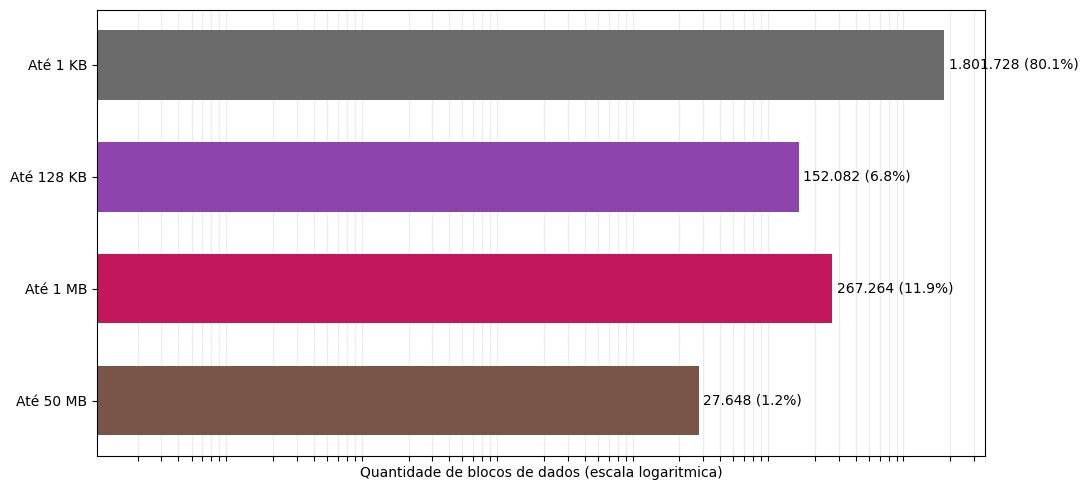
\includegraphics[width=\textwidth]{figuras/histograma_mensagens.png}
  \caption{Distribuição agregada da quantidade de blocos de dados por
  faixa de tamanho no experimento, em escala logarítmica.}
  \label{fig:histograma_mensagens}
\end{figure}

% =============================================================
\section{Experimento AWS}
\label{sec:exp_aws}

O Experimento AWS foi configurado na nuvem da Amazon Web Services (AWS),
utilizando 32 nós da instância do tipo r7i.12xlarge. Essa instância é
baseada na quarta geração de processadores Intel Xeon Scalable (Sapphire
Rapids 8488C), operando a 3,2~GHz, e disponibiliza 24 núcleos físicos com
suporte a \textit{hyper-threading}, totalizando 48 processadores lógicos.
O sistema conta ainda com 384~GB de memória DDR5, que oferece maior
largura de banda em relação às gerações anteriores, e um adaptador de
rede Ethernet com capacidade de até 18,75~Gbps, projetado para cargas de
trabalho intensivas em comunicação. Essa configuração enquadra-se na
categoria de instâncias otimizadas para memória da AWS
(\textit{memory-optimized}), adequada a aplicações que combinam elevada
demanda de processamento paralelo com grandes volumes de dados em
memória --- perfil característico do SDDP, em que cada \textit{rank} MPI
chega a consumir mais de 8~GB de memória residente. Nos experimentos,
utilizou-se a biblioteca MPICH2 versão~3.2 e um sistema de arquivos
paralelo Lustre versão~2.12 de 12~TB, com 1~MDS de 350~GB e 10~OSTs de
1,165~TB. O \textit{stripe count} foi configurado como 10, com
\textit{stripes} de 1~MB, disponibilizado por meio do serviço
Amazon FSx for Lustre. Pelos motivos discutidos na introdução do
capítulo, configurou-se um \textit{rank} por núcleo físico, totalizando
24 \textit{ranks} MPI por nó, que processam cenários em paralelo
segundo o padrão \textit{bag-of-tasks} descrito na
Subseção~\ref{sec:padrao_dados_sddp}~\cite{intel:23,aws:24}.


\subsection{Avaliação da implementação atual}
\label{sec:aws_atual}
Esta subseção analisa o desempenho da arquitetura atual de E/S do SDDP
no Experimento AWS. A Tabela~\ref{tab:central_aws} sumariza os resultados
obtidos com a base de dados PMO/PAR de outubro de 2023, considerando
1.536 cenários, três estágios mensais e 24
\textit{ranks} por nó.

Observa-se que o tempo total de execução cai com o aumento do número de
nós até 16~nós, passando de aproximadamente 8\,971~s em 2~nós para
1\,874~s em 16~nós, mas volta a crescer para 2\,013~s em 32~nós ---
caracterizando o regime saturado típico de um cenário de \textit{strong
scaling} limitado pela E/S. A banda agregada degrada-se de 60{,}5~Gb/s
em 2~nós para 3{,}4~Gb/s em 32~nós (mais de uma ordem de grandeza), e o
percentual do tempo dedicado à E/S cresce de 0{,}34\% em 2~nós para
49{,}51\% em 32~nós. Esses números são coerentes com o
diagnóstico de que o adaptador de rede do nó escritor se torna ponto de
contenção à medida que aumenta o número de processos emissores
concorrentes.

Na Tabela~\ref{tab:central_aws}, o tempo total corresponde ao tempo de
execução medido, que inclui computação, E/S e comunicação. Os tempos de
I/O e comunicação são apresentados separadamente.

\begin{table}[H]
\centering
\caption{Desempenho do Experimento AWS com a implementação atual,
incluindo tempos de I/O, comunicação, tempo total, \textit{speedup},
eficiência e percentual de I/O. A eficiência é calculada em relação à
base de 2~nós.}
\label{tab:central_aws}
\small
\setlength{\tabcolsep}{4pt}
\renewcommand{\arraystretch}{1.25}
\resizebox{\textwidth}{!}{%
\begin{tabular}{cccccccc}
\toprule
\textbf{Nós} &
\textbf{\shortstack{Banda percebida\\(Gb/s)}} &
\textbf{\shortstack{I/O\\(s)}} &
\textbf{\% I/O} &
\textbf{\shortstack{Comunicação\\(s)}} &
\textbf{\shortstack{Total\\(s)}} &
\textbf{Speedup} &
\textbf{\shortstack{Eficiência\\(\%)}} \\
\midrule
2  & $60{,}51 \pm 4{,}56$ & $30{,}85 \pm 2{,}05$ & $0{,}34\%$  & $177{,}51 \pm 26{,}06$ & $8\,971{,}23 \pm 305{,}56$ & $1{,}00\times$ & $100{,}0\%$ \\
4  & $51{,}28 \pm 2{,}48$ & $78{,}23 \pm 3{,}04$ & $1{,}62\%$  & $212{,}76 \pm 16{,}94$ & $4\,823{,}20 \pm 46{,}53$  & $1{,}86\times$ & $93{,}0\%$ \\
8  & $18{,}94 \pm 3{,}30$ & $201{,}67 \pm 4{,}13$ & $7{,}64\%$  & $174{,}04 \pm 11{,}31$ & $2\,639{,}18 \pm 16{,}07$  & $3{,}40\times$ & $85{,}0\%$ \\
16 & $4{,}52  \pm 0{,}29$ & $527{,}94 \pm 2{,}91$ & $28{,}18\%$ & $167{,}77 \pm 6{,}19$  & $1\,873{,}56 \pm 49{,}91$  & $4{,}79\times$ & $59{,}9\%$ \\
32 & $3{,}37  \pm 0{,}09$ & $996{,}57 \pm 5{,}28$ & $49{,}51\%$ & $304{,}96 \pm 3{,}36$  & $2\,013{,}06 \pm 25{,}50$  & $4{,}46\times$ & $27{,}9\%$ \\
\bottomrule
\end{tabular}
}
\end{table}

\subsection{Avaliação da implementação MPI-IO com escritas independentes}
\label{sec:aws_mpiio}
Esta subseção analisa o desempenho da arquitetura proposta, baseada em
escritas independentes com MPI-IO sobre o sistema de arquivos
Lustre, no Experimento AWS. Nesta abordagem cada processo MPI escreve seus
próprios dados diretamente no FSx for Lustre, eliminando o ponto de
contenção associado a um único processo escritor e explorando o
paralelismo dos múltiplos OSTs.

A Tabela~\ref{tab:mpiio_aws} consolida os resultados obtidos com a
implementação MPI-IO no Experimento AWS. Assim como na tabela
anterior, o tempo total corresponde ao tempo de execução medido, que
inclui computação, E/S, comunicação e Coordenação MPI-IO. Os tempos de
I/O, comunicação e Coordenação MPI-IO são apresentados separadamente; a
coordenação corresponde às chamadas
\texttt{MPI\_File\_Open}/\texttt{MPI\_File\_Close}.

\begin{table}[H]
\centering
\caption{Desempenho do Experimento AWS com a implementação MPI-IO,
incluindo tempos de I/O, comunicação, coordenação, tempo total,
\textit{speedup}, eficiência e percentual de I/O. A eficiência é
calculada em relação à base de 2~nós.}
\label{tab:mpiio_aws}
\small
\setlength{\tabcolsep}{4pt}
\renewcommand{\arraystretch}{1.25}
\resizebox{\textwidth}{!}{%
\begin{tabular}{ccccccccc}
\toprule
\textbf{Nós} &
\textbf{\shortstack{Banda percebida\\(Gb/s)}} &
\textbf{\shortstack{I/O\\(s)}} &
\textbf{\% I/O} &
\textbf{\shortstack{Comunicação\\(s)}} &
\textbf{\shortstack{Coord.\\(s)}} &
\textbf{\shortstack{Total\\(s)}} &
\textbf{Speedup} &
\textbf{\shortstack{Eficiência\\(\%)}} \\
\midrule
2  & $57{,}04 \pm 7{,}42$   & $18{,}57 \pm 0{,}86$ & $0{,}21\%$ & $188{,}65 \pm 22{,}49$ & $42{,}48 \pm 6{,}74$  & $8\,858{,}91 \pm 97{,}68$ & $1{,}00\times$ & $100{,}0\%$ \\
4  & $106{,}04 \pm 17{,}02$ & $12{,}54 \pm 0{,}38$ & $0{,}24\%$ & $233{,}95 \pm 21{,}24$ & $51{,}23 \pm 13{,}28$ & $5\,127{,}24 \pm 94{,}25$ & $1{,}73\times$ & $86{,}4\%$ \\
8  & $167{,}03 \pm 35{,}23$ & $9{,}36 \pm 0{,}32$  & $0{,}36\%$ & $186{,}69 \pm 18{,}47$ & $69{,}82 \pm 4{,}10$  & $2\,599{,}75 \pm 32{,}55$ & $3{,}41\times$ & $85{,}2\%$ \\
16 & $274{,}24 \pm 13{,}44$ & $7{,}42 \pm 0{,}10$  & $0{,}48\%$ & $233{,}77 \pm 4{,}50$  & $83{,}53 \pm 3{,}65$  & $1\,558{,}33 \pm 8{,}23$  & $5{,}68\times$ & $71{,}1\%$ \\
32 & $380{,}30 \pm 26{,}86$ & $8{,}93 \pm 0{,}08$  & $0{,}70\%$ & $236{,}02 \pm 8{,}15$  & $147{,}26 \pm 6{,}41$ & $1\,274{,}25 \pm 20{,}95$ & $6{,}95\times$ & $43{,}5\%$ \\
\bottomrule
\end{tabular}
}
\end{table}

\subsection{Análise comparativa}
\label{sec:avaliacao_comparativa_aws}
Os resultados das duas subseções anteriores são consolidados visualmente
nas figuras a seguir, que apresentam, lado a lado, os perfis de banda
agregada, tempo de execução e tempo de bloqueio de envio em função do
número de nós para as duas implementações.

A Tabela~\ref{tab:comparativo_aws} resume os principais indicadores
comparativos do Experimento AWS. A melhoria no tempo total é pequena em
2~nós, torna-se negativa em 4~nós, mas passa a ser positiva a partir de
8~nós e cresce nas maiores escalas: 1{,}5\% em 8~nós, 16{,}8\% em
16~nós e 36{,}7\% em 32~nós. A comparação de banda evidencia o principal
ganho da arquitetura proposta: a MPI-IO passa de desempenho
ligeiramente inferior em 2~nós para 2{,}07$\times$ a banda da
implementação atual em 4~nós, 8{,}82$\times$ em 8~nós, 60{,}66$\times$
em 16~nós e 113{,}00$\times$ em 32~nós. A redução do tempo de E/S também
cresce com a escala, chegando a 99{,}1\% em 32~nós.

\begin{table}[H]
\centering
\caption{Resumo comparativo entre a implementação atual e MPI-IO no
Experimento AWS. A melhoria no total e a melhoria de I/O são calculadas
em relação à implementação atual; valores negativos indicam piora.}
\label{tab:comparativo_aws}
\small
\setlength{\tabcolsep}{3pt}
\renewcommand{\arraystretch}{1.25}
\resizebox{\textwidth}{!}{%
\begin{tabular}{cccccccccc}
\toprule
\textbf{Nós} &
\textbf{\shortstack{Total\\atual (s)}} &
\textbf{\shortstack{Total\\MPI-IO (s)}} &
\textbf{\shortstack{Melhoria\\no total (\%)}} &
\textbf{\shortstack{Banda percebida\\atual (Gb/s)}} &
\textbf{\shortstack{Banda percebida\\MPI-IO (Gb/s)}} &
\textbf{\shortstack{Ganho de\\banda perc.}} &
\textbf{\shortstack{I/O\\atual (s)}} &
\textbf{\shortstack{I/O\\MPI-IO (s)}} &
\textbf{\shortstack{Melhoria\\I/O (\%)}} \\
\midrule
2  & $8\,971{,}23$ & $8\,858{,}91$ & $1{,}3\%$   & $60{,}51$ & $57{,}04$  & $0{,}94\times$   & $30{,}85$  & $18{,}57$ & $39{,}8\%$ \\
4  & $4\,823{,}20$ & $5\,127{,}24$ & $-6{,}3\%$  & $51{,}28$ & $106{,}04$ & $2{,}07\times$   & $78{,}23$  & $12{,}54$ & $84{,}0\%$ \\
8  & $2\,639{,}18$ & $2\,599{,}75$ & $1{,}5\%$   & $18{,}94$ & $167{,}03$ & $8{,}82\times$   & $201{,}67$ & $9{,}36$  & $95{,}4\%$ \\
16 & $1\,873{,}56$ & $1\,558{,}33$ & $16{,}8\%$  & $4{,}52$  & $274{,}24$ & $60{,}66\times$  & $527{,}94$ & $7{,}42$  & $98{,}6\%$ \\
32 & $2\,013{,}06$ & $1\,274{,}25$ & $36{,}7\%$  & $3{,}37$  & $380{,}30$ & $113{,}00\times$ & $996{,}57$ & $8{,}93$  & $99{,}1\%$ \\
\bottomrule
\end{tabular}
}
\end{table}

A Figura~\ref{fig:Banda_AWS} apresenta a evolução da banda agregada
média percebida pela aplicação no Experimento AWS. As duas curvas exibem comportamentos
qualitativamente opostos: a
implementação atual parte de aproximadamente 60{,}5~Gb/s em 2~nós
e degrada-se de forma acentuada com o aumento do paralelismo, atingindo
18{,}9~Gb/s em 8~nós, 4{,}5~Gb/s em 16~nós e 3{,}4~Gb/s em 32~nós ---
uma redução de mais de uma ordem de grandeza. Em contraste, a
implementação MPI-IO parte de 57{,}0~Gb/s em 2~nós e cresce
monotonicamente, alcançando 106{,}0~Gb/s em 4~nós, 167{,}0~Gb/s em
8~nós, 274{,}2~Gb/s em 16~nós e 380{,}3~Gb/s em 32~nós.

Em 2~nós, a banda agregada da implementação atual é cerca de 6\% maior
que a da implementação MPI-IO. Esse comportamento é coerente com o fato
de que, em pequena escala, o gargalo do processo escritor único ainda não
se manifesta, e o custo fixo da coordenação da E/S paralela tem maior
peso relativo. A partir de 4~nós, entretanto, a implementação MPI-IO já
supera a atual. Em 8~nós, a banda agregada é aproximadamente
$8{,}8\times$ maior; em 16~nós, cerca de $60{,}7\times$ maior; e, em
32~nós, aproximadamente $113{,}0\times$ maior. Esse resultado indica que a
arquitetura proposta explora a infraestrutura de armazenamento em uma
escala completamente diferente da arquitetura baseada em escritor único.

Essa diferença de comportamento decorre diretamente da eliminação do
processo escritor único. Na arquitetura atual, todas as escritas
convergem para o adaptador de rede de um único nó, que rapidamente se
torna ponto de contenção e limita o \textit{throughput} global ---
explicando a queda contínua da banda observada. Na abordagem MPI-IO, as operações de escrita são distribuídas entre os
processos MPI, permitindo que múltiplos fluxos de dados sejam enviados
simultaneamente ao sistema de arquivos Lustre, explorando o paralelismo
proporcionado pelos múltiplos OSTs. Como consequência, a banda agregada
cresce de forma consistente com o número de nós, demonstrando que o
sistema de armazenamento ainda não atingiu seu limite nominal na maior
configuração avaliada. Dessa forma, a figura evidencia que a adoção de
MPI-IO não apenas elimina o gargalo da arquitetura atual, mas também
permite um uso significativamente mais eficiente da largura de banda
disponível, tornando a aplicação adequada para execuções em larga escala.

\begin{figure}[H]
  \centering
  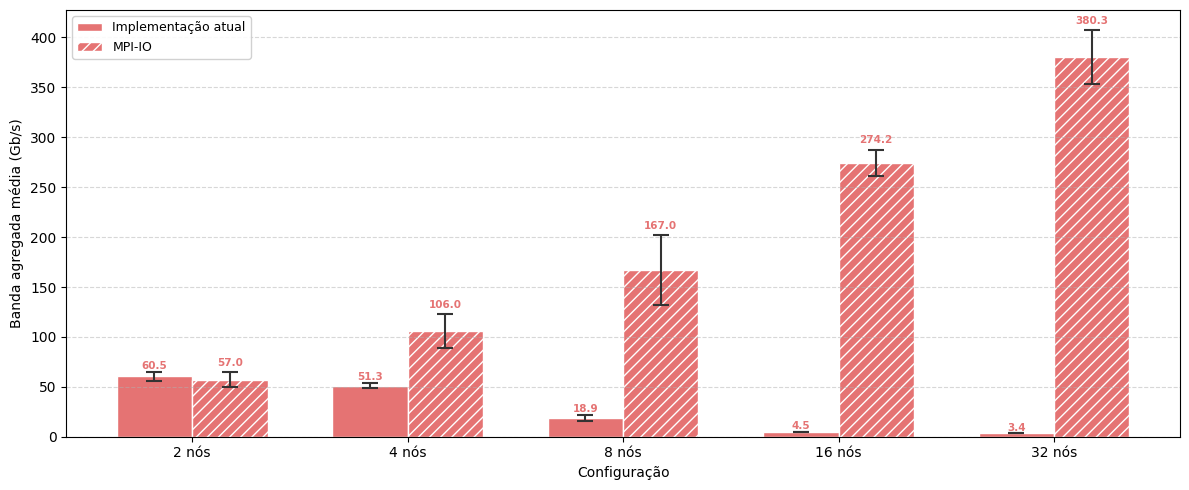
\includegraphics[width=\textwidth]{figuras/Banda_AWS.png}
  \caption{Banda agregada média percebida pela aplicação no
  Experimento AWS.}
  \label{fig:Banda_AWS}
\end{figure}

A Figura~\ref{fig:Tempo_execucao_AWS} apresenta a evolução do tempo total
de execução no Experimento AWS, contrastando a implementação atual e a
implementação MPI-IO sobre o Lustre.
As barras de erro representam apenas o desvio padrão do tempo de execução
total, e não desvios individuais das parcelas internas.
Nas configurações de menor escala, em que a E/S não é o componente
dominante, as duas curvas evoluem de forma próxima: em 2~nós,
$8{,}97 \times 10^{3}$~s no modelo atual contra $8{,}86 \times
10^{3}$~s no modelo MPI-IO; em 4~nós, entretanto, a versão MPI-IO
apresenta $5{,}13 \times 10^{3}$~s contra $4{,}82 \times
10^{3}$~s da implementação atual. Esse comportamento é coerente, uma vez
que, em pequena escala, o tempo de execução é dominado pela computação e
o custo da coordenação ainda tem maior peso relativo.

A divergência entre as duas curvas torna-se evidente a partir de 8~nós e
se acentua de forma marcante nas configurações de maior porte. Enquanto a
implementação atual apresenta um regime de saturação --- com o
tempo de execução passando de $2{,}64 \times 10^{3}$~s em 8~nós para
$1{,}87 \times 10^{3}$~s em 16~nós e voltando a crescer para
$2{,}01 \times 10^{3}$~s em 32~nós ---, a implementação MPI-IO mantém
uma redução consistente do tempo total, atingindo $2{,}60 \times
10^{3}$~s em 8~nós, $1{,}56 \times 10^{3}$~s em 16~nós e $1{,}27
\times 10^{3}$~s em 32~nós. Em termos relativos, isso corresponde a uma
redução do tempo total de aproximadamente 1{,}5\% em 8~nós, 16{,}8\% em
16~nós e 36{,}7\% em 32~nós em relação ao modelo atual.

A figura também evidencia que, na implementação atual, o
crescimento do número de nós deixa de produzir ganho de desempenho a
partir de 16~nós e passa a ser, na prática, contraproducente em 32~nós
--- comportamento característico de regime degradado sob \textit{strong
scaling}, no qual a contenção do processo escritor mais do que compensa
os ganhos de paralelismo computacional. Em contraste, a curva
MPI-IO permanece monotonicamente decrescente em todo o intervalo
avaliado, indicando que a infraestrutura de armazenamento ainda não
atingiu sua capacidade limite mesmo na maior configuração testada.

Cabe observar que, na implementação MPI-IO, o tempo de E/S torna-se uma
fração pequena do tempo total em todas as escalas, permanecendo próximo
ou abaixo de 1\% a partir de 4~nós. Na implementação atual, por outro lado, a
fração de E/S cresce de 7,6\% em 8~nós para 28,2\% em 16~nós e 49,5\%
em 32~nós. Na implementação MPI-IO, parte do tempo de simulação passa a
ser ocupada pela Coordenação MPI-IO, medida pelas chamadas
\texttt{MPI\_File\_Open}/\texttt{MPI\_File\_Close}: essa parcela cresce
de 0{,}5\% em 2~nós para 1{,}0\% em 4~nós, 2{,}7\% em 8~nós, 5{,}4\%
em 16~nós e 11{,}6\% em 32~nós. Esse crescimento percentual, contudo, reflete
sobretudo a redução do tempo de simulação com o aumento do paralelismo
e não um aumento da carga útil tratada por essas chamadas. Como
\texttt{MPI\_File\_Open}/\texttt{MPI\_File\_Close} são executadas
uma única vez por execução --- no início e no final ---, trata-se de
um \emph{overhead fixo} em relação à carga útil do problema: não
cresce com o número de cenários nem com o número de estágios
resolvidos. Esse custo, no entanto, varia com o número de nós
computacionais, já que envolve sincronização coletiva entre todos os
\textit{ranks} envolvidos na abertura do arquivo compartilhado --- e
é exatamente esse comportamento que se observa nos dados, com a
parcela absoluta crescendo de 42~s em 2~nós para 147~s em 32~nós.
Os experimentos aqui apresentados consideram
apenas três estágios mensais, o que mantém o tempo total de
simulação relativamente curto e infla a fração percentual da
Coordenação MPI-IO; em execuções de operação programada típicas do
SIN, com horizonte de vários anos e número de cenários muito maior,
o custo absoluto dessas chamadas, para uma dada configuração de nós,
permanece o mesmo enquanto o tempo total cresce em ordem de
magnitude, diluindo a parcela de coordenação para níveis
desprezíveis. A partir de 8~nós, e mesmo sob essa inflação relativa do
custo de coordenação, a implementação MPI-IO já apresenta
tempo total inferior ao da implementação atual.

\begin{figure}[H]
  \centering
  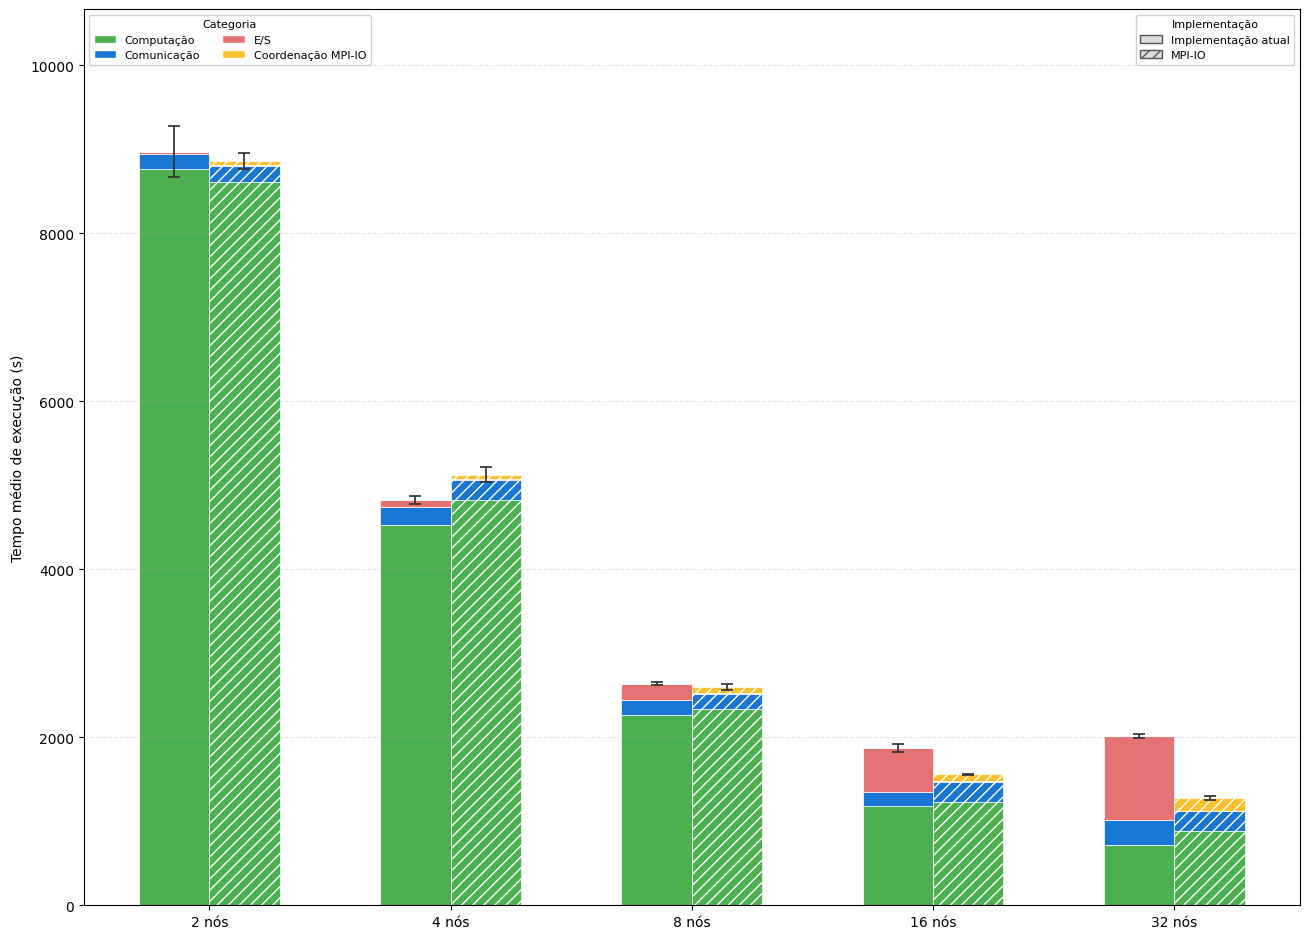
\includegraphics[width=\textwidth]{figuras/Tempo_execucao_AWS.png}
  \caption{Tempo de execução no Experimento AWS.}
  \label{fig:Tempo_execucao_AWS}
\end{figure}

A Figura~\ref{fig:EnvioPorTamanho_AWS} apresenta o tempo médio de
bloqueio das operações de E/S, em segundos, em função do tamanho dos
blocos de dados no Experimento AWS, em escala logarítmica. A comparação mostra
que, para blocos de dados muito pequenos, a implementação atual apresenta
tempos menores, pois o custo fixo das chamadas MPI-IO se torna dominante em
relação ao volume transferido. Esse efeito, contudo, ocorre em uma faixa de
tempo baixa, da ordem de microssegundos a poucos milissegundos, e não
determina o tempo total da aplicação.

Para blocos de dados médios e grandes, que concentram o impacto de E/S nas
maiores escalas, o comportamento se inverte. Em 16 e 32~nós, a
implementação atual passa a apresentar tempos de bloqueio elevados nas
classes de maior tamanho, chegando à ordem de segundos, enquanto a
implementação MPI-IO permanece na ordem de centésimos ou décimos de segundo.
Assim, a figura reforça o diagnóstico das Figuras~\ref{fig:Banda_AWS}
e~\ref{fig:Tempo_execucao_AWS}: a abordagem com escritor único é competitiva
apenas em pequena escala ou para blocos de dados muito pequenos, mas perde
escalabilidade quando o volume de dados e a concorrência entre processos
aumentam.

\begin{figure}[H]
  \centering
  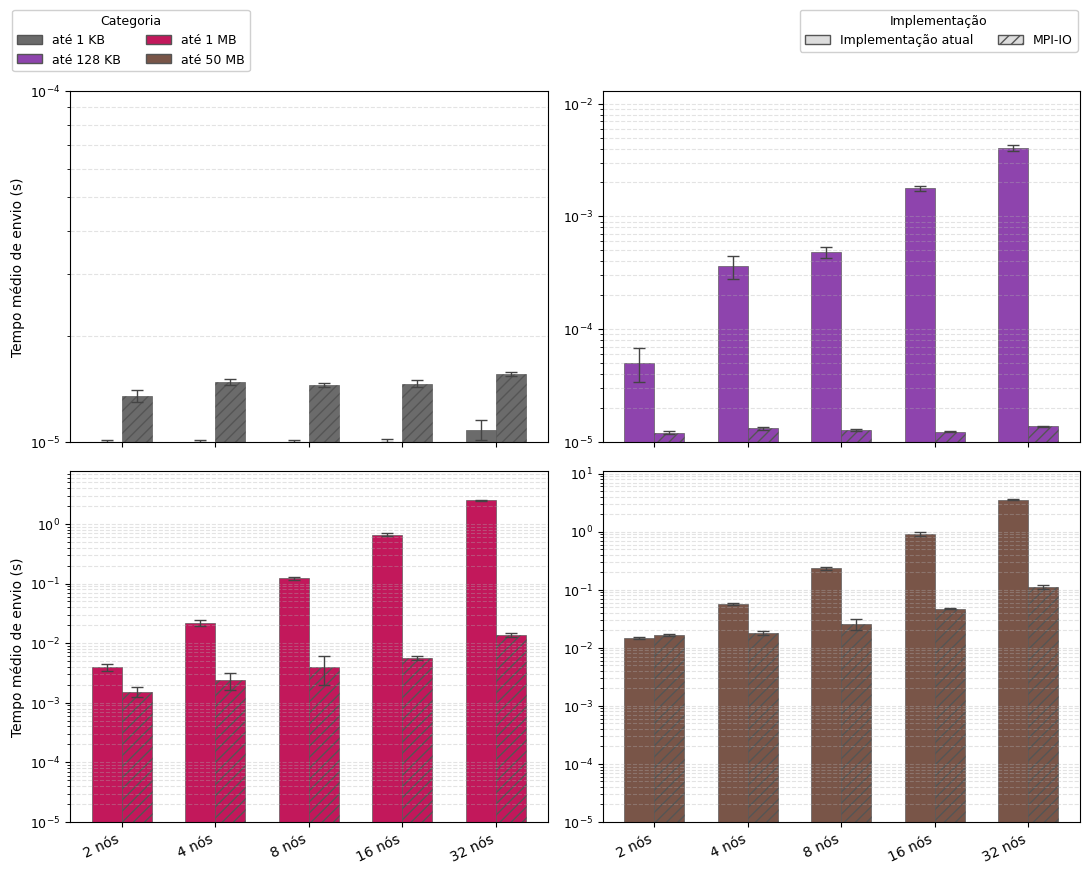
\includegraphics[width=\textwidth]{figuras/EnvioPorTamanho_AWS.png}
  \caption{Tempo médio de bloqueio das operações de envio em função do
  tamanho dos blocos de dados no Experimento AWS (escala logarítmica).}
  \label{fig:EnvioPorTamanho_AWS}
\end{figure}

% =============================================================
\subsection{Avaliação do impacto do número de OSTs}
\label{sec:exp_osts}

Esta subseção tem como objetivo avaliar, no Experimento AWS, o impacto do número de
\textit{Object Storage Targets} (OSTs) no desempenho das operações de E/S
no sistema de arquivos Lustre. Em ambientes HPC, a quantidade de OSTs
está diretamente relacionada ao grau de paralelismo de E/S disponível,
uma vez que os dados podem ser distribuídos entre múltiplos dispositivos
de armazenamento, permitindo acessos concorrentes por diferentes
processos.

A análise apresentada nesta subseção foi conduzida em rodada experimental
específica, com instrumentação dedicada à isolação do efeito do número de
OSTs. Os valores absolutos não devem ser comparados diretamente com os
das Subseções \ref{sec:aws_atual}--\ref{sec:avaliacao_comparativa_aws}
(em particular, com a Tabela~\ref{tab:mpiio_aws}); o foco aqui é a
tendência relativa entre as configurações de 4 e 10 OSTs.

Para esta avaliação, foram realizados experimentos com a abordagem
MPI-IO variando-se a quantidade de OSTs disponíveis no FSx for Lustre,
comparando configurações com 4~OSTs e 10~OSTs para execuções com 16 e
32~nós de cálculo. As demais características do experimento foram
mantidas constantes, incluindo o volume de dados e o padrão de acesso,
de modo a isolar o efeito da infraestrutura de armazenamento.

A Figura~\ref{fig:Experimento_OSTs} apresenta o tempo médio de envio
por classe de tamanho das mensagens. Cada subfigura corresponde a uma
classe de tamanho, enquanto as barras comparam as configurações MPI-IO
com 4 e 10~OSTs para 16 e 32~nós de cálculo. Em 16~nós, o uso de
10~OSTs aumenta o tempo médio de envio nas classes pequenas, de
0{,}014~ms para 2{,}1~ms nas mensagens de até 1~KB e de 0{,}014~ms para
4{,}7~ms nas mensagens de até 128~KB. Nas classes que concentram maior
volume de dados, porém, o comportamento se inverte: o tempo cai de
82{,}6~ms para 7{,}1~ms nas mensagens de até 1~MB e de 524~ms para
48~ms nas mensagens de até 50~MB.

O efeito é mais pronunciado em 32~nós, quando a maior concorrência entre
processos amplia a diferença entre as duas configurações. Nesse cenário,
as classes pequenas permanecem mais rápidas com 4~OSTs, com tempos de
0{,}018~ms nas mensagens de até 1~KB e 0{,}018~ms nas mensagens de até
128~KB, contra 3{,}2~ms e 10~ms com 10~OSTs. Para blocos maiores,
entretanto, o aumento do número de OSTs reduz o tempo médio de envio de
309~ms para 13{,}7~ms nas mensagens de até 1~MB e de 1{,}89~s para
105~ms nas mensagens de até 50~MB. Esses resultados mostram que a
redução do número de OSTs aumenta a contenção no acesso aos dados
principalmente nas classes de maior volume, sobretudo quando o número de
nós de cálculo cresce. Embora a escrita seja realizada em paralelo por
meio de MPI-IO, a disponibilidade de menos alvos de armazenamento limita
o paralelismo efetivo do Lustre e aumenta o tempo observado nas
operações de envio dessas classes.

\begin{figure}[H]
  \centering
  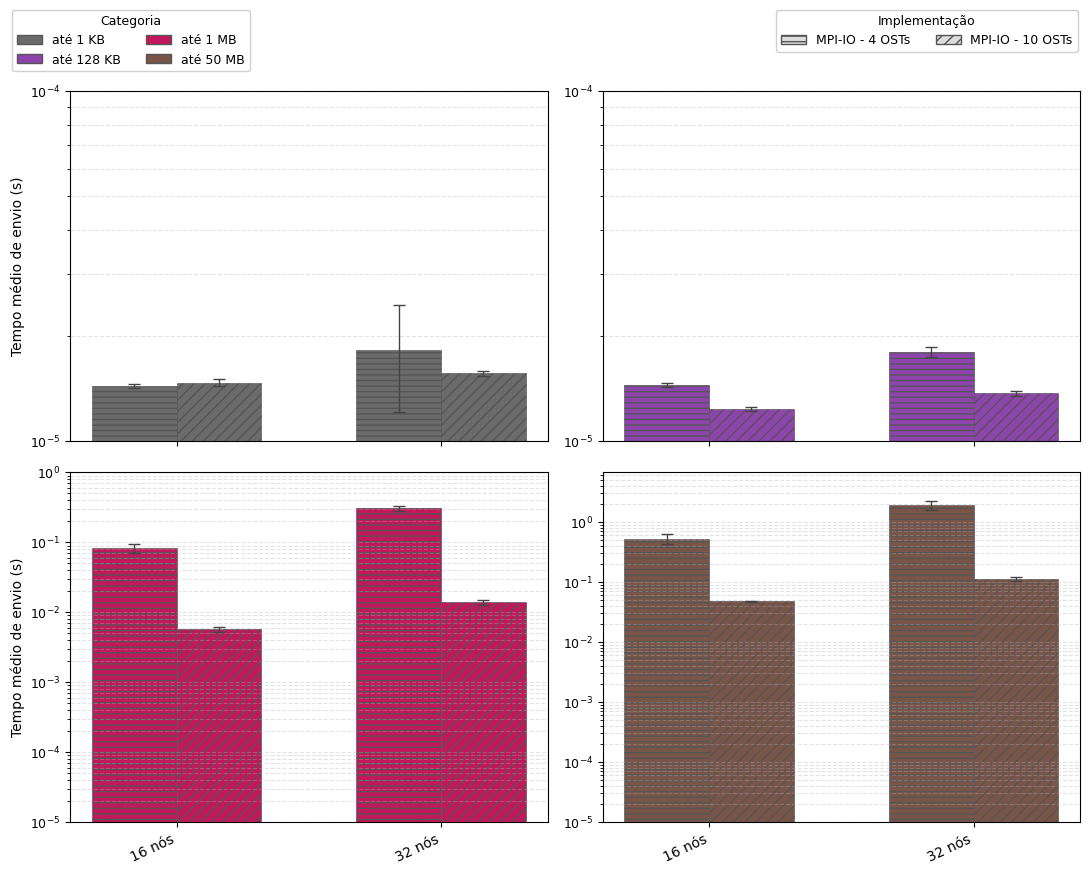
\includegraphics[width=\textwidth]{figuras/Experimento_OSTs.png}
  \caption{Tempo médio de envio por classe de tamanho das mensagens para
  configurações MPI-IO com 4 e 10~OSTs.}
  \label{fig:Experimento_OSTs}
\end{figure}

A Figura~\ref{fig:Experimento_OSTs_banda} complementa essa análise ao
apresentar a banda agregada média percebida pela aplicação em cada
configuração. Com
16~nós, a configuração com 10~OSTs atinge 274{,}2~Gb/s, contra
49{,}4~Gb/s com 4~OSTs, ganho de aproximadamente 5{,}6$\times$. Ao
passar de 16 para 32~nós, as configurações exibem tendências opostas:
com 10~OSTs, a banda cresce para 380{,}3~Gb/s, enquanto, com 4~OSTs, cai
para 16{,}1~Gb/s. Dessa forma, em 32~nós, o uso de 10~OSTs resulta em
ganho de aproximadamente 23{,}6$\times$ sobre a configuração com 4~OSTs.
Esse comportamento indica que, quando a concorrência entre processos
aumenta, a configuração com menos OSTs passa a limitar a escalabilidade
da E/S.

Assim, a análise conjunta das duas figuras indica que o aumento no
número de OSTs melhora tanto a largura de banda agregada quanto o tempo
médio das operações de envio nas classes de maior volume. A configuração
com 10~OSTs permite melhor distribuição das requisições entre os alvos de
armazenamento, enquanto a configuração com 4~OSTs concentra o tráfego em
menos dispositivos e introduz gargalos mais visíveis no cenário com
32~nós.

\begin{figure}[H]
  \centering
  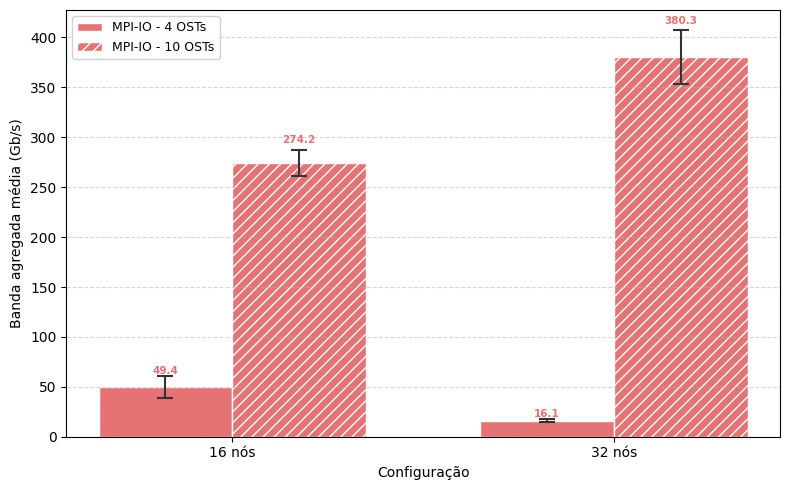
\includegraphics[width=\textwidth]{figuras/Experimento_OSTs_banda.png}
  \caption{Banda agregada média percebida pela aplicação na
  implementação MPI-IO para configurações com 4 e 10~OSTs em 16 e
  32~nós.}
  \label{fig:Experimento_OSTs_banda}
\end{figure}

% =============================================================
\section{Experimento SDumont}
\label{sec:exp_sdumont}

O Experimento SDumont corresponde ao supercomputador Santos Dumont
(SDumont), adquirido junto à empresa francesa EVIDEN/ATOS/BULL, que está
localizado na sede do Laboratório Nacional de Computação Científica
(LNCC), em Petrópolis-RJ, atuando como nó central (Tier-0) do Sistema
Nacional de Processamento de Alto Desempenho (SINAPAD). Nesse experimento
foram utilizados até 32~nós de processamento, cada um equipado com dois
processadores Intel Xeon Cascade Lake Gold 6252, totalizando 24~núcleos
físicos por nó, com suporte a \textit{hyper-threading}, o que resulta em
48~processadores lógicos disponíveis. Cada nó conta ainda com 384~GB de
memória e interconexão de alta velocidade baseada em InfiniBand EDR de
100~Gb/s, projetada para reduzir a latência e aumentar a eficiência em
aplicações paralelas de larga escala. Nos experimentos, foi utilizada a
biblioteca MPICH2 versão~3.2 e um sistema de arquivos paralelo Lustre
v2.12 implementado através do ClusterStor L300 da Cray/HPE. Essa
implementação do Lustre é composta por 1~nó MDS (com 1~MDT) e 6~nós OSSs
(cada um servindo 1~OST). O \textit{stripe count} foi configurado como 6,
com \textit{stripes} de 1~MB, disponibilizando um
espaço total de armazenamento de 1,1~PB. Pelos motivos discutidos na
introdução do capítulo, também aqui se configurou um \textit{rank} por
núcleo físico, totalizando 24 \textit{ranks} MPI por nó, que processam
cenários em paralelo segundo o padrão \textit{bag-of-tasks}.

Diferentemente do FSx for Lustre dedicado utilizado no Experimento AWS, o
sistema de arquivos do SDumont é compartilhado com outras cargas de
trabalho de HPC executando concorrentemente, o que introduz variabilidade
adicional nas medições e amplifica o efeito da contenção sobre os
recursos do sistema de arquivos nas maiores escalas. Esse compartilhamento
faz do SDumont um cenário mais desafiador para a avaliação da
escalabilidade de E/S do que o ambiente isolado da AWS.


\subsection{Avaliação da implementação atual}
\label{sec:sdumont_atual}
Esta subseção analisa o desempenho da arquitetura atual de E/S do SDDP
no Experimento SDumont. A Tabela~\ref{tab:central_sdumont} sumariza os
resultados, considerando 1.536 cenários, três estágios mensais e 24
\textit{ranks} por nó.

O tempo total de execução medido decresce com o
aumento do número de nós: 14.703~s em 2~nós, 7.572~s em 4~nós,
4.987~s em 8~nós, 2.993~s em 16~nós e 2.989~s em 32~nós. Essa redução,
contudo, perde eficiência rapidamente: o speedup passa de
1{,}94$\times$ em 4~nós para 2{,}95$\times$ em 8~nós,
4{,}91$\times$ em 16~nós e 4{,}92$\times$ em 32~nós, o que corresponde
a queda de eficiência de 97{,}1\% para 30{,}7\%. Notavelmente, o tempo
total praticamente estagna entre 16 e 32~nós (2.993~s e 2.989~s,
respectivamente), sintoma de que o gargalo da arquitetura
centralizada já se manifesta a partir de 16~nós e impede ganhos
adicionais com o aumento do paralelismo. A banda agregada percebida
confirma o diagnóstico: parte de 62{,}8~Gb/s em 2~nós, recua para
46{,}2~Gb/s em 4~nós e colapsa a partir de 8~nós, mantendo-se entre
3{,}8 e 5{,}4~Gb/s no restante da faixa avaliada. A parcela de E/S,
embutida no tempo de simulação, salta de 0{,}24\% em 2~nós para
19{,}43\% em 8~nós, 21{,}85\% em 16~nós e 39{,}98\% em 32~nós,
evidência direta de que o gargalo da arquitetura centralizada se
intensifica nas maiores escalas.

\begin{table}[H]
\centering
\caption{Desempenho do Experimento SDumont com a implementação atual. O
tempo total corresponde ao tempo de execução medido, que inclui computação,
E/S e comunicação. A eficiência é calculada em relação à base de 2~nós.}
\label{tab:central_sdumont}
\small
\setlength{\tabcolsep}{4pt}
\renewcommand{\arraystretch}{1.25}
\resizebox{\textwidth}{!}{%
\begin{tabular}{cccccccc}
\toprule
\textbf{Nós} &
\textbf{\shortstack{Banda percebida\\(Gb/s)}} &
\textbf{\shortstack{I/O\\(s)}} &
\textbf{\% I/O} &
\textbf{\shortstack{Comunicação\\(s)}} &
\textbf{\shortstack{Total\\(s)}} &
\textbf{Speedup} &
\textbf{\shortstack{Eficiência\\(\%)}} \\
\midrule
2  & $62{,}78 \pm 1{,}83$ & $34{,}73 \pm 1{,}01$       & $0{,}24\%$  & $374{,}04 \pm 13{,}10$ & $14\,702{,}88 \pm 26{,}41$ & $1{,}00\times$ & $100{,}0\%$ \\
4  & $46{,}19 \pm 3{,}15$ & $75{,}76 \pm 2{,}59$       & $1{,}00\%$  & $332{,}55 \pm 12{,}98$ & $7\,571{,}66 \pm 14{,}39$  & $1{,}94\times$ & $97{,}1\%$ \\
8  & $4{,}26 \pm 0{,}29$  & $968{,}97 \pm 6{,}94$      & $19{,}43\%$ & $385{,}68 \pm 19{,}75$ & $4\,987{,}34 \pm 77{,}08$  & $2{,}95\times$ & $73{,}7\%$ \\
16 & $5{,}37 \pm 0{,}87$  & $654{,}04 \pm 3{,}73$      & $21{,}85\%$ & $395{,}28 \pm 9{,}54$  & $2\,992{,}77 \pm 77{,}20$  & $4{,}91\times$ & $61{,}4\%$ \\
32 & $3{,}77 \pm 1{,}02$  & $1\,194{,}97 \pm 7{,}10$   & $39{,}98\%$ & $494{,}93 \pm 15{,}30$ & $2\,988{,}68 \pm 75{,}36$  & $4{,}92\times$ & $30{,}7\%$ \\
\bottomrule
\end{tabular}
}
\end{table}

\subsection{Avaliação da implementação MPI-IO com escritas independentes}
\label{sec:sdumont_mpiio}
Esta subseção analisa o desempenho da arquitetura proposta no
Experimento SDumont, baseada em escritas independentes com MPI-IO sobre o
sistema de arquivos Lustre operado pelo ClusterStor L300. A
Tabela~\ref{tab:mpiio_sdumont} consolida os resultados.

Na implementação MPI-IO, o tempo total decresce ao longo de toda a
faixa avaliada: 15.096~s em 2~nós, 7.912~s em 4~nós, 4.151~s em
8~nós, 2.619~s em 16~nós e 2.133~s em 32~nós. Em comparação com a
implementação atual, a versão MPI-IO apresenta pequeno sobrecusto em
2 e 4~nós (aumento de 2{,}7\% e 4{,}5\%, respectivamente), mas passa
a reduzir o tempo total a partir de 8~nós, com ganhos de 16{,}8\%,
12{,}5\% e 28{,}6\% em 8, 16 e 32~nós. A banda agregada do
\textit{layer} de escrita, ao contrário do que ocorre na implementação
atual, cresce de forma consistente com o paralelismo: de 5{,}5~Gb/s
em 2~nós para 8{,}9~Gb/s em 4~nós, 12{,}1~Gb/s em 8~nós,
18{,}9~Gb/s em 16~nós e 34{,}1~Gb/s em 32~nós. O tempo médio de E/S
por processo cai de 320~s em 2~nós para 61{,}6~s em 32~nós, e a
parcela percentual de E/S no tempo de simulação permanece abaixo de
5\% em todas as configurações.

\begin{table}[H]
\centering
\caption{Desempenho do Experimento SDumont com a implementação MPI-IO. O
tempo total corresponde ao tempo de execução medido, que inclui computação,
E/S, comunicação e Coordenação MPI-IO. A eficiência é calculada em relação
à base de 2~nós.}
\label{tab:mpiio_sdumont}
\small
\setlength{\tabcolsep}{4pt}
\renewcommand{\arraystretch}{1.25}
\resizebox{\textwidth}{!}{%
\begin{tabular}{ccccccccc}
\toprule
\textbf{Nós} &
\textbf{\shortstack{Banda percebida\\(Gb/s)}} &
\textbf{\shortstack{I/O\\(s)}} &
\textbf{\% I/O} &
\textbf{\shortstack{Comunicação\\(s)}} &
\textbf{\shortstack{Coord.\\(s)}} &
\textbf{\shortstack{Total\\(s)}} &
\textbf{Speedup} &
\textbf{\shortstack{Eficiência\\(\%)}} \\
\midrule
2  & $5{,}55 \pm 0{,}33$  & $320{,}27 \pm 10{,}78$ & $2{,}12\%$ & $352{,}81 \pm 7{,}54$  & $23{,}24 \pm 2{,}65$   & $15\,096{,}47 \pm 40{,}60$  & $1{,}00\times$ & $100{,}0\%$ \\
4  & $8{,}89 \pm 0{,}85$  & $270{,}52 \pm 4{,}45$  & $3{,}42\%$ & $231{,}00 \pm 11{,}26$ & $32{,}27 \pm 1{,}40$   & $7\,912{,}23 \pm 81{,}80$   & $1{,}91\times$ & $95{,}4\%$ \\
8  & $12{,}09 \pm 1{,}33$ & $193{,}57 \pm 2{,}23$  & $4{,}66\%$ & $222{,}57 \pm 6{,}92$  & $79{,}31 \pm 19{,}18$  & $4\,151{,}01 \pm 124{,}19$  & $3{,}64\times$ & $90{,}9\%$ \\
16 & $18{,}85 \pm 1{,}04$ & $99{,}41 \pm 0{,}95$   & $3{,}79\%$ & $281{,}28 \pm 16{,}08$ & $126{,}49 \pm 24{,}82$ & $2\,619{,}43 \pm 88{,}31$   & $5{,}76\times$ & $72{,}0\%$ \\
32 & $34{,}10 \pm 4{,}70$ & $61{,}61 \pm 0{,}78$   & $2{,}89\%$ & $357{,}72 \pm 19{,}57$ & $230{,}03 \pm 7{,}78$  & $2\,132{,}82 \pm 75{,}89$   & $7{,}08\times$ & $44{,}2\%$ \\
\bottomrule
\end{tabular}
}
\end{table}

\subsection{Análise comparativa}
\label{sec:avaliacao_comparativa_sdumont}
Os resultados das duas subseções anteriores são consolidados visualmente
nas figuras a seguir, que apresentam, lado a lado, os perfis de banda
agregada, tempo de execução e tempo de bloqueio de envio em função do
número de nós para as duas implementações no Experimento SDumont.

A Tabela~\ref{tab:comparativo_sdumont} resume os principais indicadores
comparativos do Experimento SDumont. A coluna de melhoria no tempo total
compara diretamente a implementação MPI-IO com a implementação atual para
o mesmo número de nós, calculada como
$(Total_{atual} - Total_{MPIIO})/Total_{atual}$. Valores positivos
indicam redução do tempo total, enquanto valores negativos indicam piora.
A MPI-IO apresenta sobrecusto em pequena escala (--2{,}7\% em 2~nós e
--4{,}5\% em 4~nós), mas passa a reduzir o tempo total a partir de
8~nós, com ganhos de 16{,}8\%, 12{,}5\% e 28{,}6\% em 8, 16 e
32~nós. O ganho de banda também cresce nas maiores escalas: alcança
2{,}83$\times$ em 8~nós, 3{,}51$\times$ em 16~nós e 9{,}05$\times$
em 32~nós. A redução do tempo médio de E/S chega a 80{,}0\% em
8~nós, 84{,}8\% em 16~nós e 94{,}8\% em 32~nós, atestando que a
contenção do escritor único é o fator dominante de degradação da
implementação atual nessas escalas.

\begin{table}[H]
\centering
\caption{Resumo comparativo entre a implementação atual e MPI-IO no
Experimento SDumont. A melhoria no total e a melhoria de I/O são
calculadas em relação à implementação atual; valores negativos indicam
piora.}
\label{tab:comparativo_sdumont}
\small
\setlength{\tabcolsep}{3pt}
\renewcommand{\arraystretch}{1.25}
\resizebox{\textwidth}{!}{%
\begin{tabular}{cccccccccc}
\toprule
\textbf{Nós} &
\textbf{\shortstack{Total\\atual (s)}} &
\textbf{\shortstack{Total\\MPI-IO (s)}} &
\textbf{\shortstack{Melhoria\\no total (\%)}} &
\textbf{\shortstack{Banda percebida\\atual (Gb/s)}} &
\textbf{\shortstack{Banda percebida\\MPI-IO (Gb/s)}} &
\textbf{\shortstack{Ganho de\\banda perc.}} &
\textbf{\shortstack{I/O\\atual (s)}} &
\textbf{\shortstack{I/O\\MPI-IO (s)}} &
\textbf{\shortstack{Melhoria\\I/O (\%)}} \\
\midrule
2  & $14\,702{,}88$ & $15\,096{,}47$ & $-2{,}7\%$  & $62{,}78$ & $5{,}55$  & $0{,}09\times$ & $34{,}73$  & $320{,}27$ & $-822{,}2\%$ \\
4  & $7\,571{,}66$  & $7\,912{,}23$  & $-4{,}5\%$  & $46{,}19$ & $8{,}89$  & $0{,}19\times$ & $75{,}76$  & $270{,}52$ & $-257{,}1\%$ \\
8  & $4\,987{,}34$  & $4\,151{,}01$  & $16{,}8\%$  & $4{,}26$  & $12{,}09$ & $2{,}83\times$ & $968{,}97$ & $193{,}57$ & $80{,}0\%$ \\
16 & $2\,992{,}77$  & $2\,619{,}43$  & $12{,}5\%$  & $5{,}37$  & $18{,}85$ & $3{,}51\times$ & $654{,}04$ & $99{,}41$  & $84{,}8\%$ \\
32 & $2\,988{,}68$  & $2\,132{,}82$  & $28{,}6\%$  & $3{,}77$  & $34{,}10$ & $9{,}05\times$ & $1\,194{,}97$ & $61{,}61$  & $94{,}8\%$ \\
\bottomrule
\end{tabular}
}
\end{table}

A Figura~\ref{fig:Banda_SDumont} compara a banda agregada média
percebida pela aplicação
obtida pela implementação atual e pela implementação MPI-IO. Em 2 e
4~nós, a implementação atual apresenta a maior banda observada, com
62{,}8~Gb/s e 46{,}2~Gb/s respectivamente, enquanto a MPI-IO atinge
5{,}5~Gb/s e 8{,}9~Gb/s --- comportamento esperado em pequena
escala, em que o custo fixo da camada MPI-IO ainda não é amortizado
pelo paralelismo de escrita. A partir de 8~nós, o quadro se inverte:
a banda da implementação atual colapsa para 4{,}3~Gb/s e a MPI-IO
sobe para 12{,}1~Gb/s --- ganho de 2{,}83$\times$. Em 16~nós, a
implementação atual permanece nesse patamar baixo, com 5{,}4~Gb/s,
enquanto a MPI-IO continua crescendo e alcança 18{,}9~Gb/s --- ganho
de 3{,}51$\times$. Em 32~nós, a diferença se acentua: a implementação
atual cai para 3{,}8~Gb/s, enquanto a MPI-IO atinge 34{,}1~Gb/s,
ganho de 9{,}05$\times$.

Mais relevante que o valor absoluto é o contraste de
\emph{comportamento}: a implementação atual exibe queda abrupta entre
4 e 8~nós e permanece em um patamar baixo nas escalas subsequentes
(entre 3{,}8 e 5{,}4~Gb/s), sintoma da saturação do escritor central
sob o Lustre compartilhado do SDumont. A implementação MPI-IO, em
contrapartida, apresenta perfil monotonicamente crescente de banda,
indicando que a infraestrutura de armazenamento ainda é capaz de
absorver maior paralelismo de escrita.

\begin{figure}[H]
  \centering
  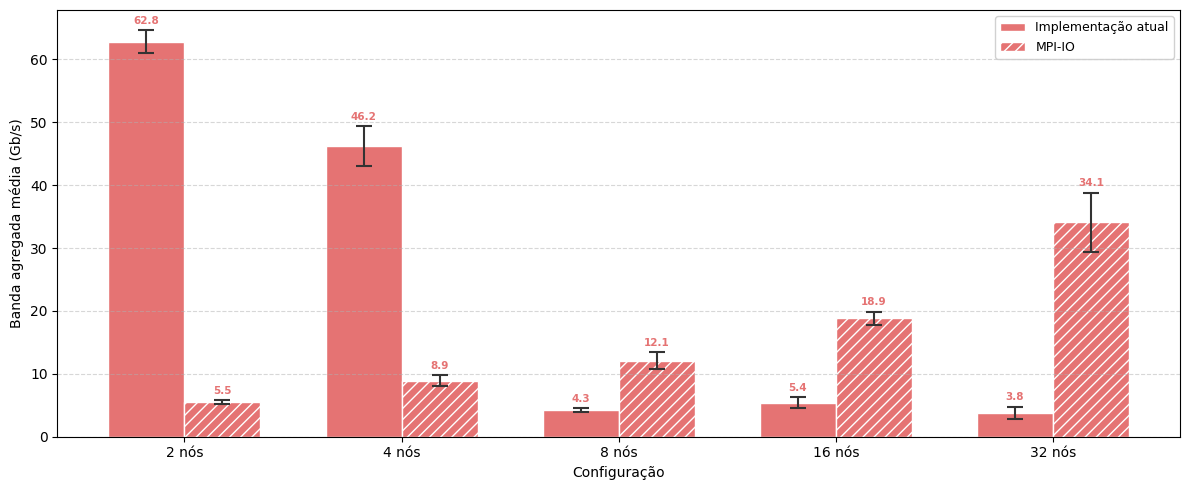
\includegraphics[width=\textwidth]{figuras/Banda_SDumont.png}
  \caption{Banda agregada média percebida pela aplicação nas
  implementações atual e MPI-IO no Experimento SDumont.}
  \label{fig:Banda_SDumont}
\end{figure}

A Figura~\ref{fig:Tempo_execucao_SDumont} detalha o tempo médio por
processo no Experimento SDumont, separando as parcelas de computação,
comunicação, E/S e Coordenação MPI-IO. A parcela Coordenação MPI-IO
corresponde às chamadas
\texttt{MPI\_File\_Open}/\texttt{MPI\_File\_Close}, executadas
\emph{uma única vez} por execução --- na abertura e no fechamento do
arquivo de saída. Trata-se, portanto, de um \emph{overhead fixo} em
relação à carga útil do problema: não cresce com o número de
cenários nem com o número de estágios resolvidos. Esse custo, no
entanto, varia com o número de nós computacionais, já que envolve
sincronização coletiva entre todos os \textit{ranks} envolvidos na
abertura do arquivo compartilhado. As
barras de erro indicam somente o desvio padrão do tempo de execução
total. Em 2 e 4~nós, a implementação MPI-IO apresenta tempo total
levemente superior ao da implementação atual: o custo das operações
de coordenação e da própria camada MPI-IO ainda pesa nessas escalas,
em que a contenção do escritor único da implementação atual ainda
não saturou. A partir de 8~nós, a versão MPI-IO reduz o tempo total
em relação à implementação atual, chegando a 28{,}6\% de redução em
32~nós.

Na implementação atual, a parcela de E/S cresce de forma marcante a
partir de 8~nós, chegando a representar uma fatia significativa do
tempo de simulação. Esse comportamento é compatível com a saturação
do processo escritor centralizado no Lustre compartilhado do
SDumont. Na implementação MPI-IO, o tempo de E/S é redistribuído
entre os processos e permanece reduzido em todas as escalas
(abaixo de 5\% do tempo de simulação), enquanto o custo da
Coordenação MPI-IO passa a compor uma fração visível do tempo total
nas maiores configurações --- em particular, cresce de cerca de
23~s em 2~nós para 126~s em 16~nós e 230~s em 32~nós.

É importante destacar que a fração relativa da Coordenação MPI-IO
observada nestes experimentos é maior do que se espera em execuções
reais do SDDP. Como já discutido, trata-se de um overhead fixo em
relação à carga útil do problema --- não cresce com o número de
cenários nem com o número de estágios resolvidos ---, de modo que
sua participação no tempo total decresce à medida que a carga
computacional aumenta. Nas execuções aqui realizadas, com apenas
três estágios mensais e $1\,536$ cenários, o tempo total de
simulação é relativamente baixo, o que infla o peso percentual dessa
parcela. Em execuções de operação programada típicas do SIN, com
horizonte de vários anos em resolução mensal e número de cenários
muito maior, o custo absoluto de coordenação, para uma dada
configuração de nós, permanece o mesmo enquanto o tempo total de
computação cresce em ordem de magnitude
--- diluindo a fração relativa da Coordenação MPI-IO para níveis
desprezíveis. Assim, a figura evidencia que a abordagem proposta
reduz o gargalo centralizado de escrita; o custo residual de
coordenação, embora visível na escala dos experimentos, não é uma
limitação intrínseca da arquitetura proposta.

\begin{figure}[H]
  \centering
  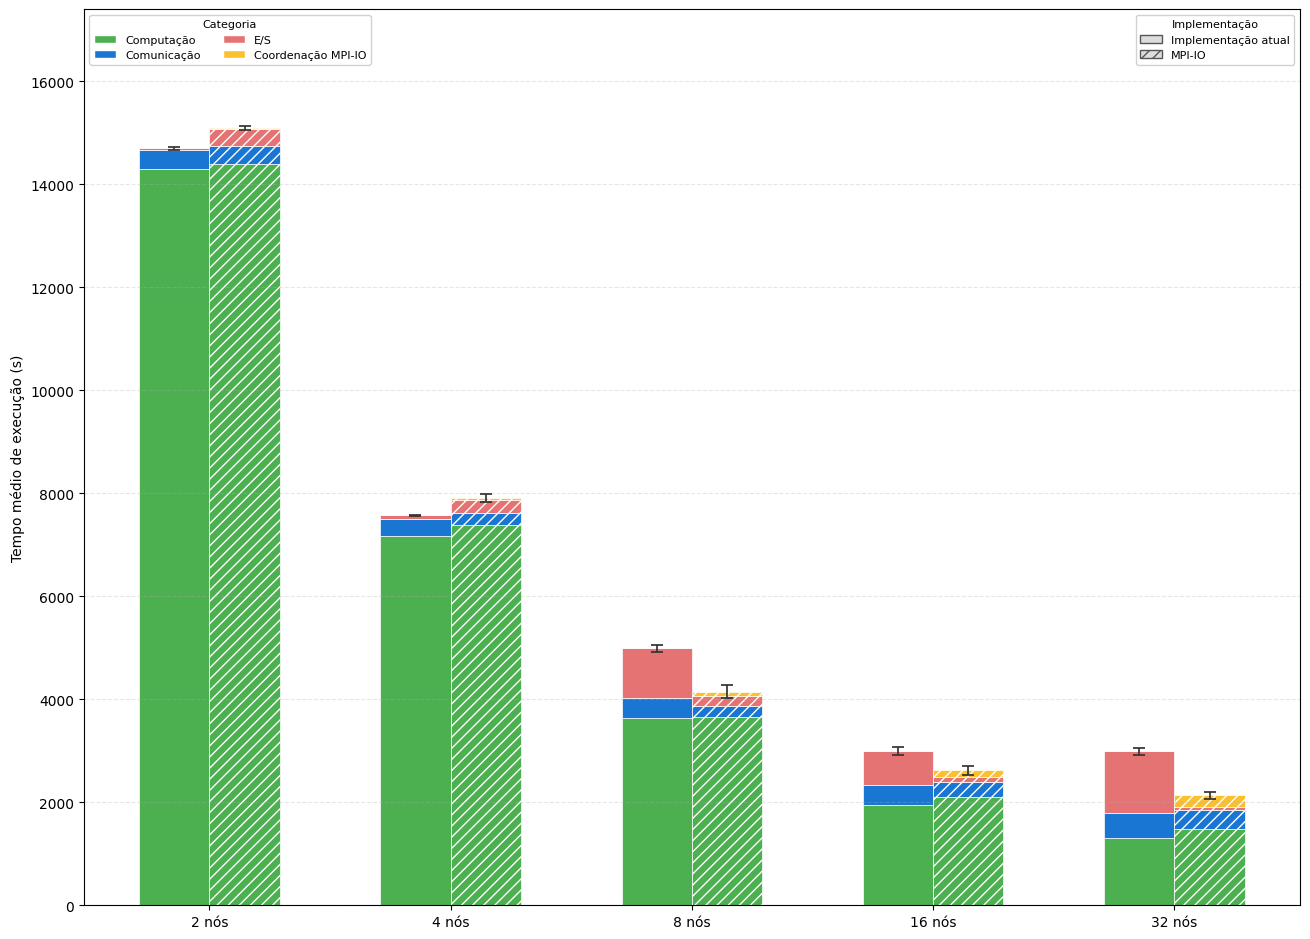
\includegraphics[width=\textwidth]{figuras/Tempo_execucao_SDumont.png}
  \caption{Decomposição do tempo médio por processo das implementações
  atual e MPI-IO no Experimento SDumont.}
  \label{fig:Tempo_execucao_SDumont}
\end{figure}

A Figura~\ref{fig:EnvioPorTamanho_SDumont} apresenta o tempo médio
de bloqueio das operações de envio em função do tamanho dos blocos
de dados no Experimento SDumont, em escala logarítmica, organizada
em quatro painéis --- um por categoria de tamanho.

O painel (a), correspondente a blocos de até 1~KB, mostra tempos de
envio na ordem de poucas dezenas de microssegundos para ambas as
implementações em todas as escalas, com diferenças marginais. Para
essa granularidade, dominada por chamadas de controle e protocolo,
nem o gargalo do escritor único nem o custo fixo da camada MPI-IO
se manifestam de forma significativa.

O painel (b), referente a blocos de até 128~KB, evidencia o
contraste mais dramático da figura. A implementação atual cresce de
$5{,}7\!\times\!10^{-5}$~s em 2~nós para $2{,}7\!\times\!10^{-3}$~s
em 8~nós e $4{,}1\!\times\!10^{-3}$~s em 32~nós, enquanto a
implementação MPI-IO permanece estável em torno de
$1{,}3\!\times\!10^{-5}$~s em todas as configurações. Nessa faixa, a
contenção do processo escritor da arquitetura atual amplifica-se
rapidamente com a concorrência, e a escrita paralela da MPI-IO chega a
apresentar vantagem de mais de duas ordens de grandeza em 32~nós.

Os painéis (c) e (d), referentes a blocos de até 1~MB e até 50~MB,
mostram um comportamento misto. Em 2 e 4~nós, a implementação atual
ainda apresenta tempos menores --- 4{,}6~ms e 21~ms na classe de
até 1~MB; 14~ms e 55~ms na classe de até 50~MB ---, enquanto a
MPI-IO paga seu custo fixo (45~ms, 71~ms, 123~ms e 250~ms,
respectivamente). Essa vantagem inicial se inverte a partir de
8~nós: a saturação do escritor único na implementação atual eleva o
tempo médio para 0{,}593~s na classe de até 1~MB e 0{,}982~s na
classe de até 50~MB, contra 0{,}094~s e 0{,}433~s da MPI-IO. Em
16~nós, a vantagem da MPI-IO consolida-se: 0{,}082~s vs.\
0{,}797~s na classe de até 1~MB (uma ordem de grandeza) e
0{,}586~s vs.\ 1{,}36~s na classe de até 50~MB. Em
32~nós, a implementação atual volta a se degradar, chegando a
2{,}90~s na classe de até 1~MB e 5{,}16~s na classe de até 50~MB,
enquanto a MPI-IO permanece em 0{,}095~s e 0{,}791~s,
respectivamente.

Em conjunto, os painéis evidenciam um ponto de troca em função da
escala: em 2 e 4~nós, a implementação atual é competitiva ou
superior em blocos médios e grandes; a partir de 8~nós, a
arquitetura MPI-IO se torna sistematicamente vantajosa em todas as
classes não triviais, com ganhos de até duas ordens de grandeza nos
blocos de até 128~KB. Esse padrão também explica diretamente o
colapso da banda agregada da implementação atual mostrado na
Figura~\ref{fig:Banda_SDumont}: a partir de 8~nós, a maior parte do
volume escrito sofre saturação no escritor único.

\begin{figure}[H]
  \centering
  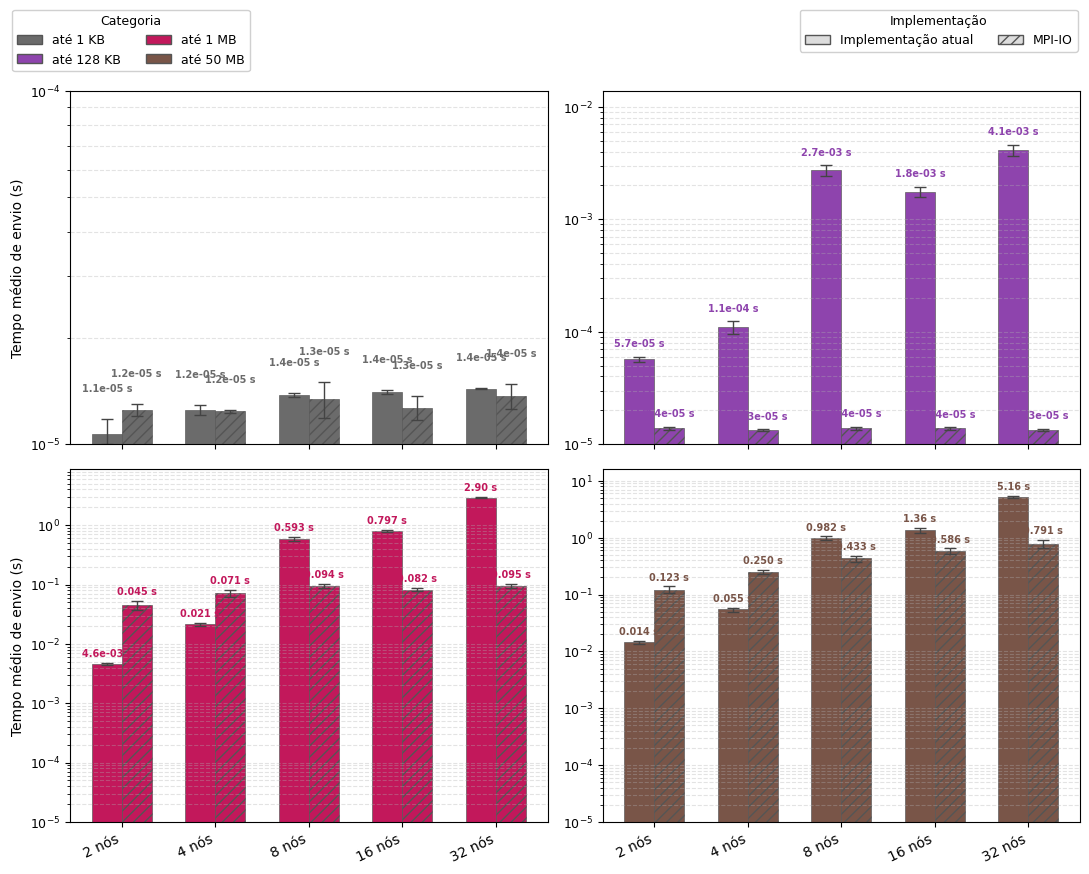
\includegraphics[width=\textwidth]{figuras/EnvioPorTamanho_SDumont.png}
  \caption{Tempo médio de bloqueio das operações de envio por tamanho de
  bloco de dados nas implementações atual e MPI-IO no Experimento SDumont
  (escala logarítmica).}
  \label{fig:EnvioPorTamanho_SDumont}
\end{figure}

Os resultados apresentados nesta seção demonstram que a adoção da
abordagem MPI-IO com escritas independentes endereça o gargalo da
arquitetura original associado à concentração das operações de E/S
no processo escritor. No SDumont, esse benefício se manifesta a
partir de 8~nós: a banda agregada cresce monotonicamente até
34{,}1~Gb/s em 32~nós, contra um perfil que colapsa e satura na
implementação atual; o tempo de E/S é reduzido em 80{,}0\%, 84{,}8\%
e 94{,}8\% em 8, 16 e 32~nós, respectivamente. Em 2 e 4~nós, o
custo fixo da camada MPI-IO ainda sobrepõe-se ao ganho de
paralelismo de escrita, e a implementação atual é ligeiramente mais
rápida. A partir de 8~nós, a MPI-IO também reduz o tempo total, com
ganho crescente até 28{,}6\% em 32~nós.

A queda de eficiência paralela observada em 32~nós --- 30{,}7\% na
implementação atual e 44{,}2\% na MPI-IO --- e a variabilidade
observada refletem, em boa medida, o caráter compartilhado do
Lustre do SDumont, em que diferentes cargas de HPC concorrem
simultaneamente pelo mesmo sistema de arquivos. Mesmo nesse cenário
hostil, o contraste qualitativo entre o perfil monotonicamente
crescente de banda da MPI-IO e o colapso da implementação atual a
partir de 8~nós persiste em toda a faixa avaliada, indicando que a
vantagem estrutural da escrita paralela se mantém quando a
infraestrutura impõe limites significativos.

% =============================================================
\section{Síntese das avaliações}
\label{sec:sintese_avaliacoes}

Os dois experimentos --- AWS, em ambiente de nuvem com FSx for Lustre
dedicado, e SDumont, em supercomputador com Lustre compartilhado
entre múltiplas cargas de HPC --- convergem para um diagnóstico
comum, ainda que com magnitudes diferentes. Em pequena escala (2 e
4~nós), a implementação atual é competitiva ou ligeiramente
superior, pois o gargalo do escritor único ainda não saturou e o
custo fixo da camada MPI-IO pesa em relação ao tempo total. A partir
de 8~nós, o quadro de E/S se inverte: a banda agregada da
implementação atual colapsa e satura, refletindo a contenção sobre
o adaptador de rede do nó escritor, enquanto a MPI-IO exibe perfil
monotonicamente crescente de banda. Esse contraste
qualitativo de comportamento --- e não apenas o ganho pontual em uma
ou outra escala --- é o resultado mais robusto deste capítulo.

A magnitude do benefício, no entanto, depende fortemente da
infraestrutura de armazenamento subjacente. No FSx for Lustre
dedicado da AWS, a abordagem proposta atinge 380{,}3~Gb/s em 32~nós
(ganho de 113$\times$ sobre a implementação atual) e reduz o tempo
total em até 36{,}7\%, com curva de banda ainda em crescimento. No
Lustre compartilhado do SDumont, a banda da MPI-IO chega a
34{,}1~Gb/s em 32~nós (ganho de 9{,}1$\times$), a redução do tempo
de E/S chega a 94{,}8\% e o tempo total cai até 28{,}6\%. Esses ganhos
ocorrem em condições adversas de concorrência por metadados e por
banda do sistema de arquivos com outras aplicações em execução. A
preservação da vantagem estrutural mesmo nesse regime sugere que a
arquitetura proposta é portátil entre ambientes heterogêneos, e não
dependente das condições idealizadas de uma plataforma dedicada.

A análise do impacto do número de OSTs na AWS reforça que o
paralelismo de armazenamento subjacente é parte essencial do ganho:
sair de 4 para 10~OSTs amplia a banda agregada em aproximadamente
5{,}6$\times$ em 16~nós e 23{,}6$\times$ em 32~nós, além de reduzir o
tempo médio das escritas nas classes de bloco maiores. Essa observação
sugere que, em deployments futuros, o dimensionamento da camada de
armazenamento --- número de OSTs e largura de \textit{stripe} ---
deve ser tratado como parâmetro de projeto, e não como detalhe
operacional.

Esses resultados não esgotam, porém, o estudo da escalabilidade da
fase de simulação final do SDDP. A faixa avaliada estendeu-se até
32~nós na AWS e no SDumont; configurações maiores podem revelar
comportamentos adicionais, em particular saturação de metadados ou
efeitos de coordenação coletiva. O custo da
Coordenação MPI-IO, que aqui se mostrou desprezível em valor
absoluto mas inflado em participação percentual pelo tamanho
reduzido das execuções de teste, merece reavaliação em cargas reais
de operação programada do SIN, com horizontes plurianuais. Por fim,
o trabalho restringiu-se à fase de simulação final, em que cenários
são mutuamente independentes; a aplicabilidade da estratégia à fase
de convergência, com seu padrão diferente de comunicação e
sincronização, fica como tema natural de continuidade.
